%%%%%%%%%%%%%%%%%%%%%%%%%%%%%%%%%%%%%%%%%%%%%%%%%%%%%%%%%%%%%%%
%
% Welcome to Overleaf --- just edit your LaTeX on the left,
% and we'll compile it for you on the right. If you open the
% 'Share' menu, you can invite other users to edit at the same
% time. See www.overleaf.com/learn for more info. Enjoy!
%
%%%%%%%%%%%%%%%%%%%%%%%%%%%%%%%%%%%%%%%%%%%%%%%%%%%%%%%%%%%%%%%
\documentclass[border=2pt]{standalone}

% Drawing
\usepackage{tikz}

% Tikz Library
\usetikzlibrary{calc, shapes}

% Styles
\tikzstyle{ray} = [line width = 0.85, color = red]
\tikzstyle{vertical} = [line width = 0.85, dashed]

% Newcommand			
\newcommand{\lline}[4]{\draw[vertical] (#1) -- ({#2*cos(#4)-#3*sin(#4)},{+#2*sin(#4)+#3*cos(#4)});}

\usetikzlibrary{backgrounds}

\begin{document}
		
	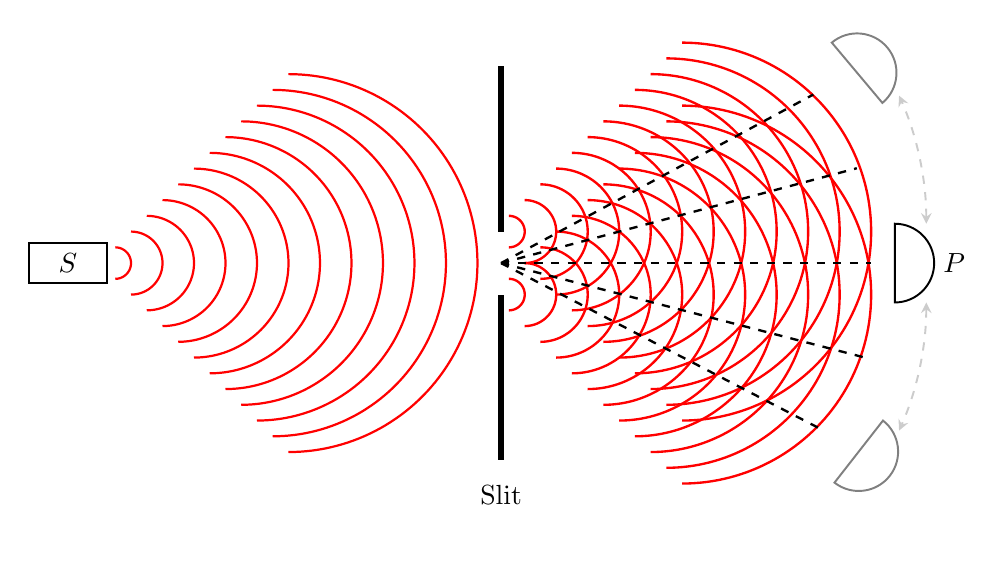
\begin{tikzpicture}[semic/.style args={#1,#2}{semicircle,minimum width=#1,draw,anchor=arc end,rotate=#2},outer sep=0pt,line width=.7pt]
		
		% Grid
%		\draw[dotted] (0,0) grid (11,4);
%		\foreach \i in {0,...,10}
%		{
%			\node at (-2ex,\i) {\i};
%			\node at (\i,-2ex) {\i};
%		}
		
		% Coordinates
		\coordinate (S) at (0.5,1);
		\coordinate (P) at (11,1.5);
		\coordinate (A) at (6,1);
		
		% Nodes
		\node[draw, rectangle, minimum width=1cm, minimum height=0.5cm] at (S) {$S$};
		\node (p') [semic={1cm,-90}, label={[rotate=0, below left, yshift=-0.7cm, black!50]}, black!50, rotate= 40] at (10.2,3.8) {};
		\node (p) [semic={1cm,-90}, label={[rotate=0]$P$}] at (P) {};
		\node (p'') [semic={1cm,-90}, label={[rotate=0, below left, yshift=-0.7cm, black!50]}, black!50, rotate= -38] at (10.85,-1.) {};
		
		% Slit
		\draw[line width = 2] (6,3.5) -- (6,1.4);
		\draw[line width = 2] (6,-1.5) -- (6,0.6) node[below, pos=-0.1] {Slit};
		
		% Dashed Grey Lines
		\draw[stealth-stealth, black!20, dashed] (11.4,1.5) arc (0:24:4);
		\draw[stealth-stealth, black!20, dashed] (11.4,0.5) arc (0:-24:4);
		
		% Interference Pattern
		%% Before Slit
		\foreach \i in {0,0.2,...,2.2}
		{
			\draw [red,thick,domain=-90:90, samples=100] plot ({0.2*cos(\x)+\i*cos(\x)+1.1+\i}, {0.2*sin(\x)+\i*sin(\x)+1});
		}
		% After Slit
		\foreach \i in {0,0.2,...,2.2}
		{
			\draw [ray, domain=-90:90, samples=100] plot ({0.2*cos(\x)+\i*cos(\x)+6.1+\i}, {0.2*sin(\x)+\i*sin(\x)+1.4});

			\draw [ray, domain=-90:90, samples=100] plot ({0.2*cos(\x)+\i*cos(\x)+6.1+\i}, {0.2*sin(\x)+\i*sin(\x)+0.6});
		}
		
		% Black Dashed Lines
		\draw[vertical] (6,1) -- (10.7,1);
		\lline{6,1}{10.7}{1}{6.5}
		\lline{6,1}{10.4}{1}{12}
		\lline{6,1}{10.6}{1}{-6.5}
		\lline{6,1}{10.1}{1}{-12}
	\end{tikzpicture}
	
\end{document}